\begin{enumerate}
  \item La fonction $\varphi$ est une fraction rationnelle dérivable dans $\R\setminus\{2\}$
\begin{displaymath}
  \varphi'(t) = \frac{2t+1}{t-2} - \frac{t^2+t}{(t-2)^2}
  = \frac{t^2-4t-2}{(t-2)^2}
  = \frac{(t-2-\sqrt{6})(t-2+\sqrt{6})}{(t-2)^2}
\end{displaymath}
On en déduit le tableau de variations.
\begin{center}
\begin{tabular}{ccccccccc}
  $-\infty$ &            & $2-\sqrt{6}$ &            & 2    &            &$2+\sqrt{6}$ &            & $+\infty$ \\ \hline 
            & $+$        &     $0$      & $-$        & $||$ & $-$        &     $0$     & $+$        &           \\ \hline
            & $\nearrow$ &     $|$      & $\searrow$ & $||$ & $\searrow$ &     $|$     & $\nearrow$ &           \\ \hline
\end{tabular}
\end{center}
La droite d'équation $x=2$ est une asymptote verticale du graphe. 

\begin{figure}[h]
  \centering
  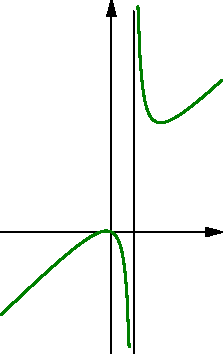
\includegraphics{./Celem16_1.pdf}
  \caption{Graphe de $\varphi$}
  \label{fig: Celem16_1}
\end{figure}

Les valeurs de la fonction aux points où la dérivée s'annule seront utiles
\begin{displaymath}
  f(2-\sqrt{6}) = 5-2\sqrt{6}\text{ (noté $u$)},\hspace{1cm}
  f(2+\sqrt{6}) = 5+2\sqrt{6} \text{ (noté $v$)}
\end{displaymath}
  \item L'équation $\mathcal{E}_m$ admet une solution dans $\R$ si et seulement si il existe un réel $x$ tel que
\begin{multline*}
\cos(2x) + 2(1-m)\cos x +1 +4m = 0 \Leftrightarrow
(2\cos x -4)m = \cos(2x) + 2\cos x + 1 \\
\Leftrightarrow
(2\cos x -4)m = 2\cos^2 x + 2\cos x 
\Leftrightarrow
(\cos x -2)m = \cos^2 x + \cos x \Leftrightarrow m = \varphi(\cos x)
\end{multline*}
On en conclut que l'équation admet une solution si et seulement si $m\in \varphi([-1,1])$.

  \item D'après l'étude de la fonction présentée dans la question précédente, la fonction $\varphi$ est
\begin{itemize}
  \item croissante dans $[-1,2-\sqrt{6}]$ de la valeur $\varphi(-1)=0$ à la valeur $u$,
  \item décroissante dans $[2-\sqrt{6},1]$ de la valeur $u$ à la valeur $\varphi(1)=-2$. 
\end{itemize}
\begin{figure}[h]
  \centering
  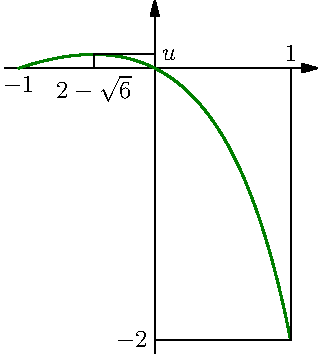
\includegraphics{./Celem16_2.pdf}
  \caption{Agrandissement du graphe de $\varphi$ dans $[-1,1]$.}
  \label{fig: Celem16_2}
\end{figure}
On en déduit que $\varphi([-1,1]= \left[-2,u \right]$.\newline
Pour chaque $t\in [-1,1]$, il existe exactement un $x\in[0,\pi]$ tel que $\cos x = t$ (à savoir $x=\arccos t$). On peut donc discuter du nombre de solutions dans $[0,\pi]$ en présentant les résultats dans un tableau.\bigskip
\begin{center}\renewcommand{\arraystretch}{1.3}
\begin{tabular}{|l|c|c|c|c|c|} \hline
  condition sur $m$:  & $m < -2$ & $-2 \leq m < 0$ & $0 \leq m < u$ & $m = u$ & $m > u$\\ \hline
  nombre de solutions:& $0$      & $1$             & $2$            & $1$     & $0$     \\ \hline
\end{tabular}
\end{center}
Remarquons bien que ce n'est pas le théorème des valeurs intermédiaires qui justifie cette discussion mais la tableau de variations établi dans la première question.

\end{enumerate}
